\documentclass{article}
\usepackage{a4wide}
\usepackage{norsk}
\usepackage{amsmath}
\usepackage{amssymb}
\usepackage{dsfont}
%\usepackage[dvips]{epsfig}
%\usepackage{graphicx}
\usepackage{fancyhdr}
\usepackage{listings}
\usepackage{nomencl}
\usepackage[pdftex]{graphicx}

\pagestyle{fancy}
\lhead{\footnotesize \parbox{11cm}{Andreas Johann H\"ormer (753179)}}
\rhead{\footnotesize {Laboratory 3}}
\chead{\footnotesize {TTT4170}}

\title{Loudspeaker Measurement (Lab 3)}
\author{Andreas Johann H\"ormer}
\date{14.02.2014}

\begin{document}
\thispagestyle{empty}
\maketitle
\thispagestyle{empty}
%\\[5cm]
\begin{center}
TTT4170 Audio Technology\\[3cm]
Lab group:
\begin{itemize}
\item Andreas Johann H\"ormer
\item Milan Stojkovic
\item Andreas Ulvoen\\[3cm]
\end{itemize}
Report delivered: \\[6cm]
FACULTY OF INFORMATION TECHNOLOGY, MATHEMATICS AND ELECTRICAL ENGINEERING\\
NORWEGIAN UNIVERSITY OF SCIENCE AND TECHNOLOGY
\end{center}
\thispagestyle{empty}
\tableofcontents
\thispagestyle{empty}
\newpage
\section*{Summary}
\thispagestyle{empty}
This report regards to the third laboratory exercise of Audio Technology at NTNU. In this laboratory a loudspeaker was measured in an anechoic room. The measurement was done in three different ways.\\
In the first task a microphone was placed in front of a loudspeaker at a distance of 1.2m. The influence of the length of the impulse time window was analyzed. It can be obtained that the frequency response get more and more smoothened when decreasing the time window size, but especially at low frequencies the results may be wrong. With full time window the frequency response is shown in a way which is expected for loudspeakers.\\
In the second measurement the loudspeaker was turned with a turntable in $15^\circ$-steps. The influence of directivity at different angles should be measured. It could be obtained, that the loudspeaker becomes more and more directional with increasing frequency, while at low frequencies the loudspeaker is more or less omnidirectional.\\
At the last measurement the influence of a reflecting surface was measured. Constructive and destructive interferences can be obtained at some frequencies.
\newpage
\setcounter{page}{1}
\section{Introduction}
Most music reproduction is done using loudspeakers. For optimal listening experience a constant quality of these reproduction devices is mandatory to ensure high listening quality. Therefore measurement of loudspeaker parameters is important to ensure high listening experience.\\
Some parameters for defining the quality of a loudspeaker are the directivity (given as directivity index DI or directivity factor DF) and the frequency response of the loudspeaker. Using the directivity, an optimal placement of the speakers to the listener can be found. The frequency response tells how the different frequencies are amplified or dampened from the speaker.\\
In this laboratory exercise the measurement of the frequency response and the directivity of a loudspeaker should be measured. This is done in three different exercises, which each of them covers a specific part of the parameter. In the first exercise the general influence of measurement parameters should be obtained. Therefore a sine sweep was recorded and the influence of the FFT window length should be obtained. In a second measurement the directivity of the loudspeaker was measured with recording sine sweeps in different off-axis angles. In the last measurement the inflluence of reflections on the measurement were obtained with placing a reflective surface between loudspeaker and measurement microphone.
\section{Theory}
\subsection{Sensitivity, Efficiency}
In loudspeakers most energy is not transformed into sound power but into heat. The efficiency is defined as the relation of transmitted sound power and the total electrical power input. It can be written as
\begin{equation}
\eta=\frac{W_{sound,out}}{W_{el,in}}
\end{equation}
Typical values for loudspeaker efficiency are 1-2\% while horn loudspeakers or high efficient loudspeakers can get up to 10\%.\\
Instead of the effiency often the loudspeakers sensitivity is listened by manufacturers. The sensitivity is defined as sound pressure level at 1W electrical input at a measurement distance of 1m. A typical voltage level for this measurement is $V_{RMS}=2.83V$. This defines the input power of 1W at a speaker impedance of $8\Omega$, which is a quite common loudspeaker impedance level. 
\subsection{Maximum output level}
For an optimal listening experience or public sound reproduction places the maximum reachable output level often should be known. This maximum output level can be calculated using following formula:
\begin{equation}
L_{P,max}=L_W+10\cdot log\bigg(\frac{DF}{4\pi\cdot r^2}+\frac{4}{A}\bigg)
\end{equation}
where
\begin{itemize}
\item $L_{P,max}$: maximum sound power level
\item $L_W$: sound power level
\item $A$: room asorption (calculation using Sabine's formula)
\item $DF$: directivity factor
\item $r$: distance from sound source
\end{itemize}
\subsection{Measurement distance}
Measurements should be done in the far field, so it must be ensured that the distance of the measurement microphone is within this distance. This is often critical around the crossover frequency, where low-frequency and mid/high-frequency elements are radiating equally strong. The critical distance can be calculated using the Rayleigh-distance, using following formula:
\begin{equation}
R_R=\frac{\pi\cdot a^2}{\lambda}
\end{equation}
where
\begin{itemize}
\item $a$: diameter of the radiating loudspeaker membrane
\item $\lambda$: radiated wavelength 
\end{itemize}
\subsection{Impulse response}
To determine the quality of a loudspeaker the impulse response and so the amplification of different frequencies has to be measured. Often this is done in an anechoic chamber, but can also be done in ordinary rooms. Then the measured impulse response has to be cut before the first wall reflections occur. Therefore the time distance between direct sound and first reflections has to be long enough.\\
The lowest frequency which can be measured accurately is defined by
\begin{equation}
\frac{1}{\Delta t}
\end{equation}
with 
\begin{itemize}
\item $\Delta t = t_{first\,reflection}-t_{direct}$
\end{itemize}
\section{Measurements}
\subsection{Equipment}
For this laboratory exercise following equipment was used:
\begin{itemize}
\item 1 measurement microphone: Norsonic 1201/30517
\item 1 loudspeaker: Genelec 1029A
\item 1 laser distance meter: Bosch PLR30
\item 1 loudspeaker turntable
\item Software:
\begin{itemize}
\item WinLMS 2004
\item Matlab 2012b
\end{itemize}
\end{itemize}

\subsection{Influence of the time window size}
The time window size defines how many fourier coefficients for the calculation of the frequency response are covered. The longer the used time window is the higher is the accuracy of the resulting frequency response. To obtain this one measurement with a microphone in front of a loudspeaker was done. A frequency sweep was recorded and the response was calculated using WinLMS. After this four different frequency responses with different time windows were created. The used time windows were 
\begin{itemize}
\item full time window
\item 3ms after the initial response
\item 10ms 
\item 50ms.
\end{itemize}
\begin{figure}[htbp]
\begin{center}
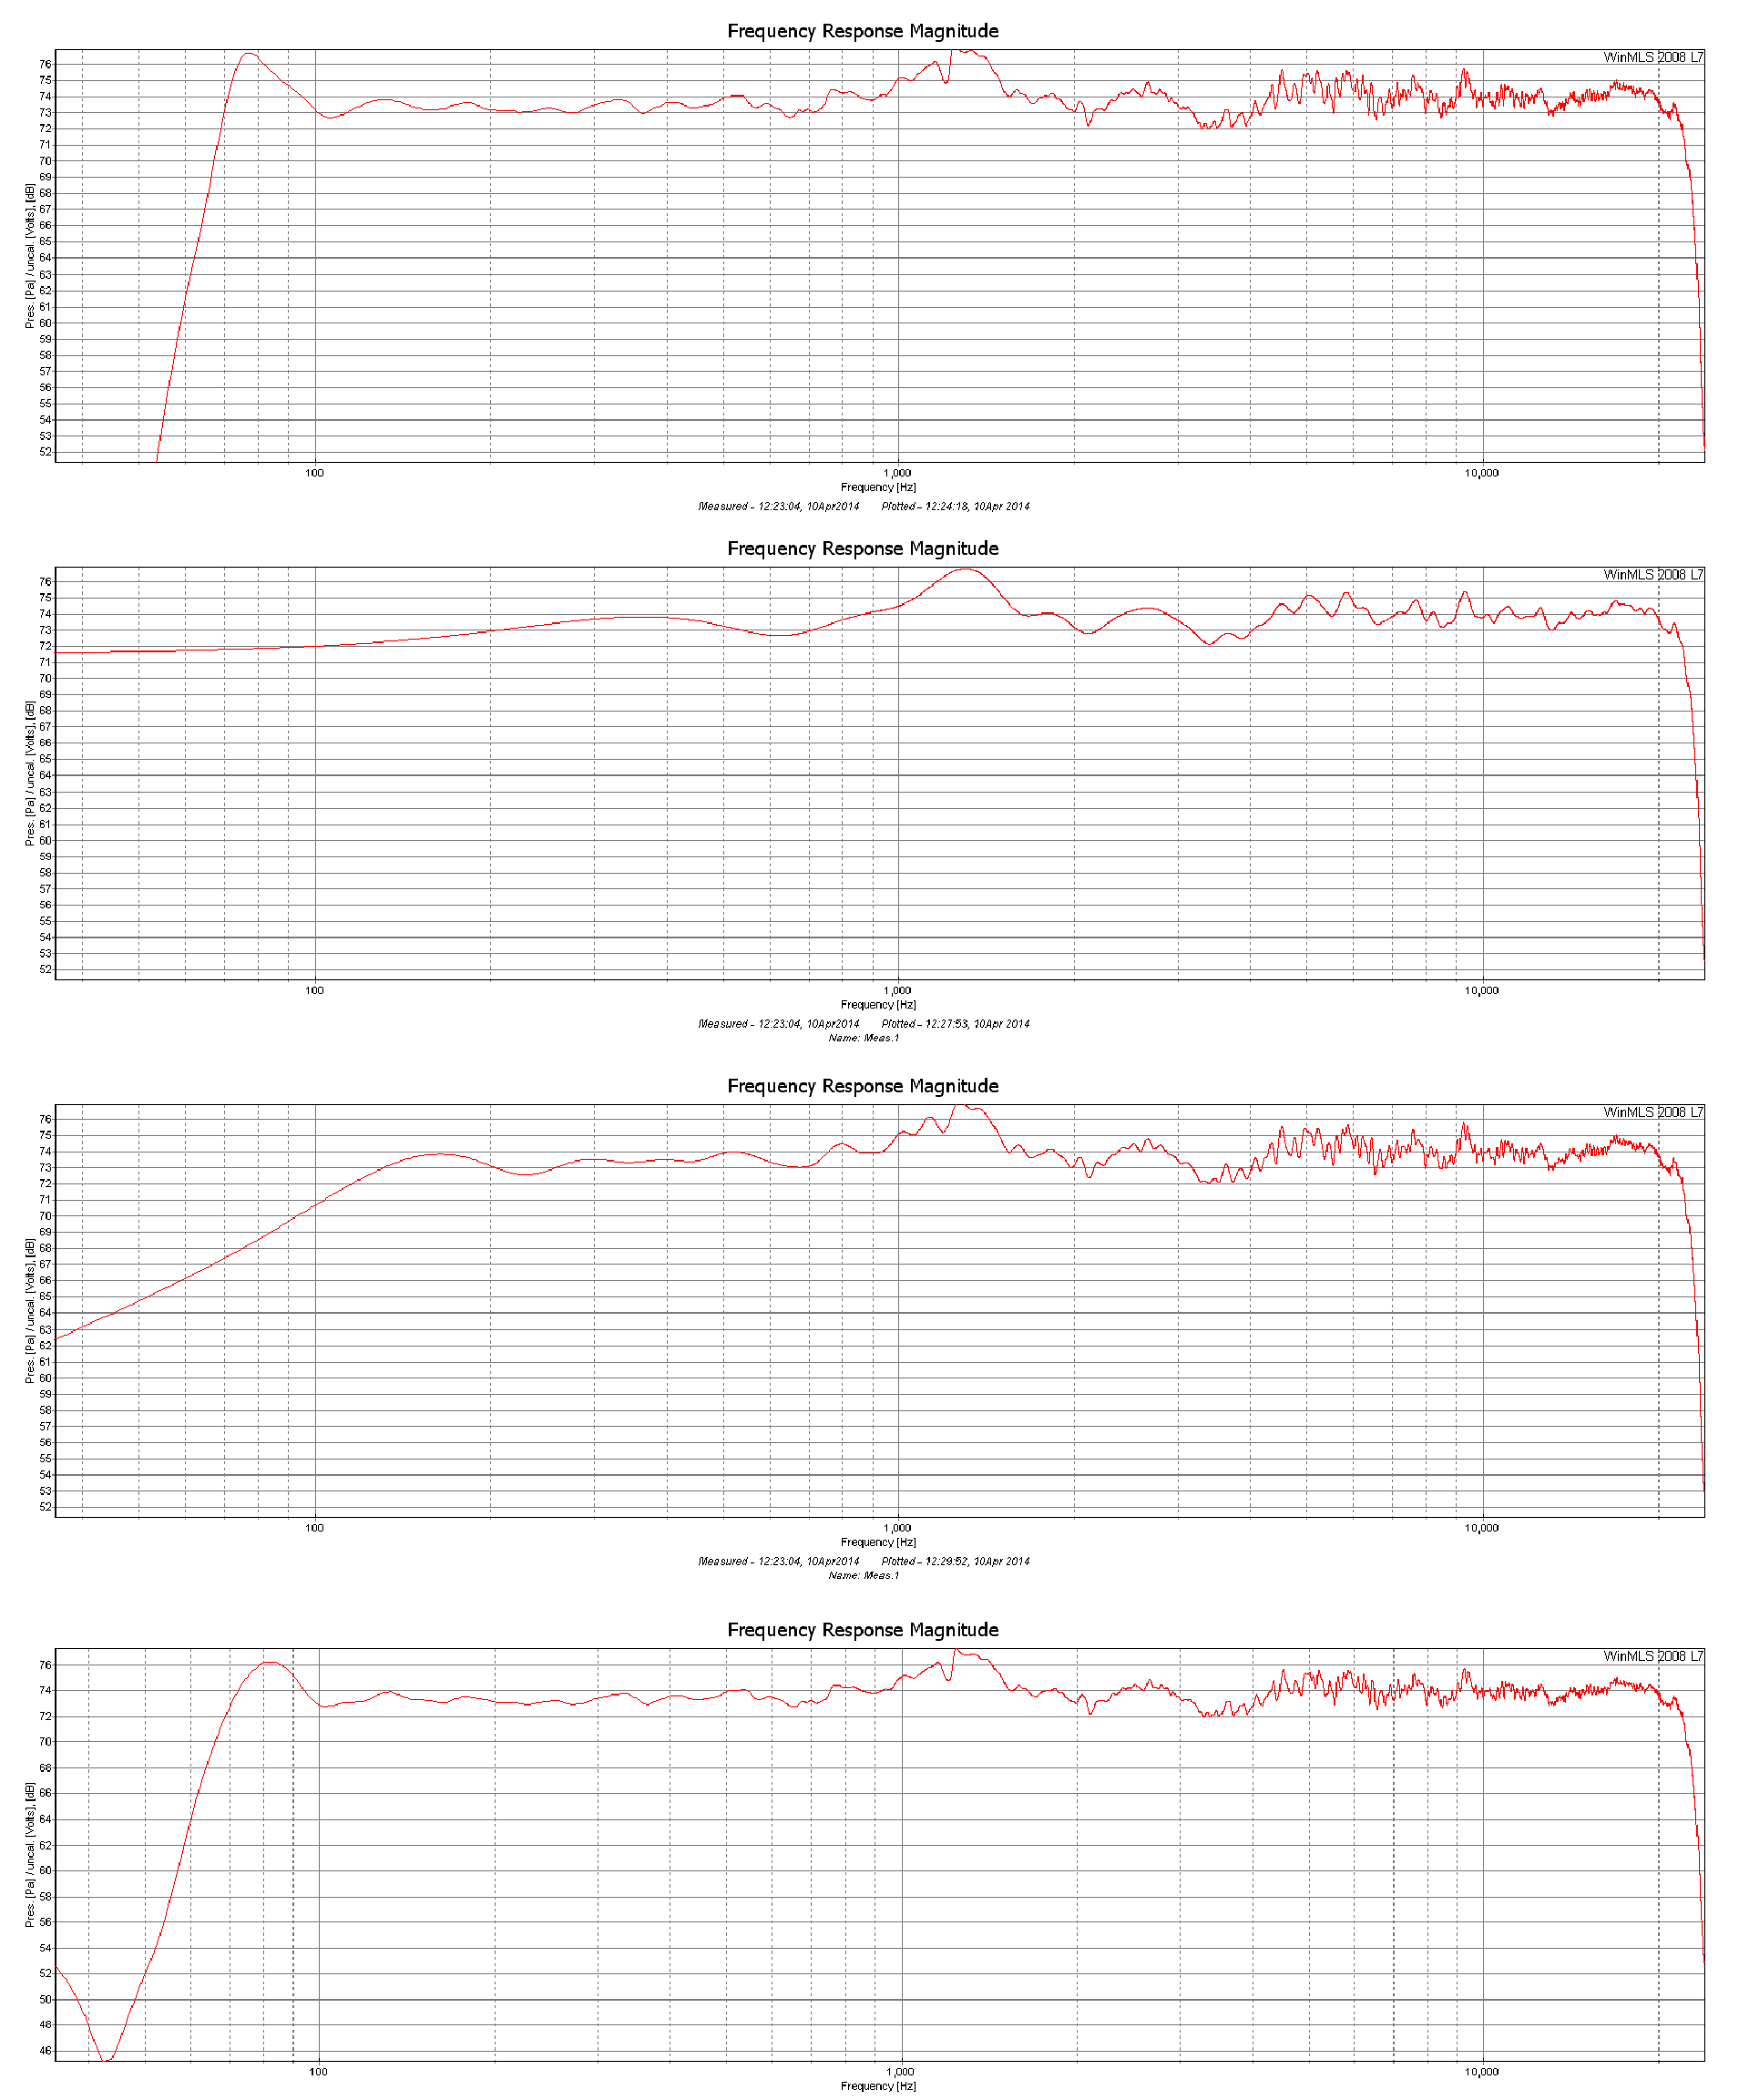
\includegraphics[width=15cm,keepaspectratio=true]{Figures/TaskAcombined}
\caption{Frequency response with (a) full time window, (b) 3ms, (c) 10ms and (d) 50ms window length}
\label{fig:TaskAcombined}
\end{center}
\end{figure}
The measured frequency responses can be seen in figure \ref{fig:TaskAcombined}.
It can be obtained that the smaller the time window size the more smooth the resulting frequency is. This is quite accurate for high frequencies where more coefficients for calculating the frequency response exist. Especially at very low frequencies it can be seen, that the result differs quite much depending on the length of the time window. For a length of 3ms or 10ms the results can not be used, because it can be seen that they are wrong. The frequency response for 50ms is quite useful and near to the result with full time window.
\subsection{Influence of incidence angle}
In an anechoic chamber (almost) no reflections should occur. So this fits perfectly for measuring the directivity of a loudspeaker. For this measurement a loudspeaker was put on a turntable, a measurement microphone in front. The speaker was turned in $15^\circ$ steps, in every step a frequency sweep was measured and the frequency response calculated using WinLMS. The different measurements were then compared together.\\
\begin{figure}[htbp]
\begin{center}
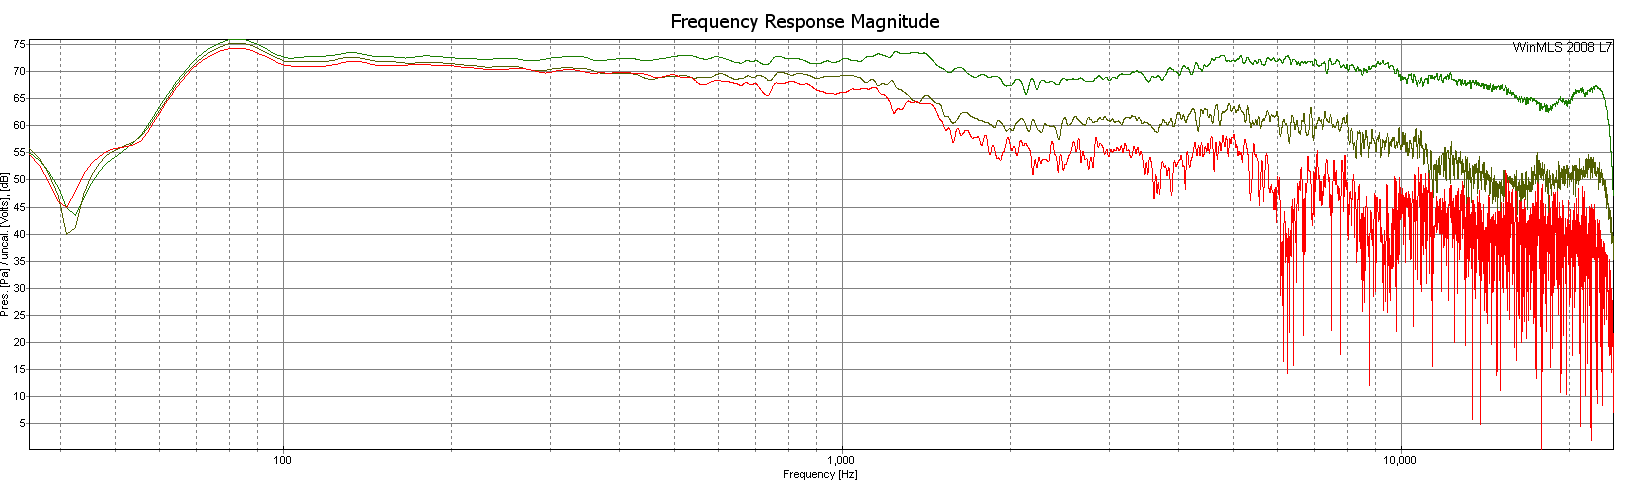
\includegraphics[width=15cm,keepaspectratio=true]{Figures/TaskBcomparison}
\caption{Directivity for $45^\circ$, $90^\circ$ and $180^\circ$ off-axis measurement}
\label{fig:TaskBcomparison}
\end{center}
\end{figure}
A comparison of different frequency responses for different incident angles can be found in figure \ref{fig:TaskBcomparison}. All measurements in $15^\circ$ steps are listed in Appendix B.1.
Here it can be seen that at low frequencies the sound propagates almost omnidirectional in each direction. When the frequency increases, the loudspeaker gets more and more directional. That can be seen at decreasing amplitudes and more reflections in the frequency response. The more the loudspeaker gets off-axis and the higher the frequency, the more the sound amplitude decreases.
\subsection{Influence of reflecting surfaces}
In this measurement the frequency response of the loudspeaker on axis should be compared to a new measurement with reflective surfaces. For this reason a wooden plate was placed on the floor between the loudpeaker and the measurement microphone. The measurement was done with a frequency sweep. Comparing the frequency response with reflections and the one without (listed in Figure \ref{fig:TaskC}) huge differences can be seen.Thi is because of strong constructive and destructive interferences between the direct sound signal from the speaker to the microphone and those frequency components which are reflected from the reflective surface.  It also can be obtained, that the influence is stronger at low frequencies, where the difference between constructive and destructive interference is almost 15dB, while at higher frequencies more interferences occur, but with less intensity. At very high frequencies the difference is about 1dB.
\begin{figure}[htbp]
\begin{center}
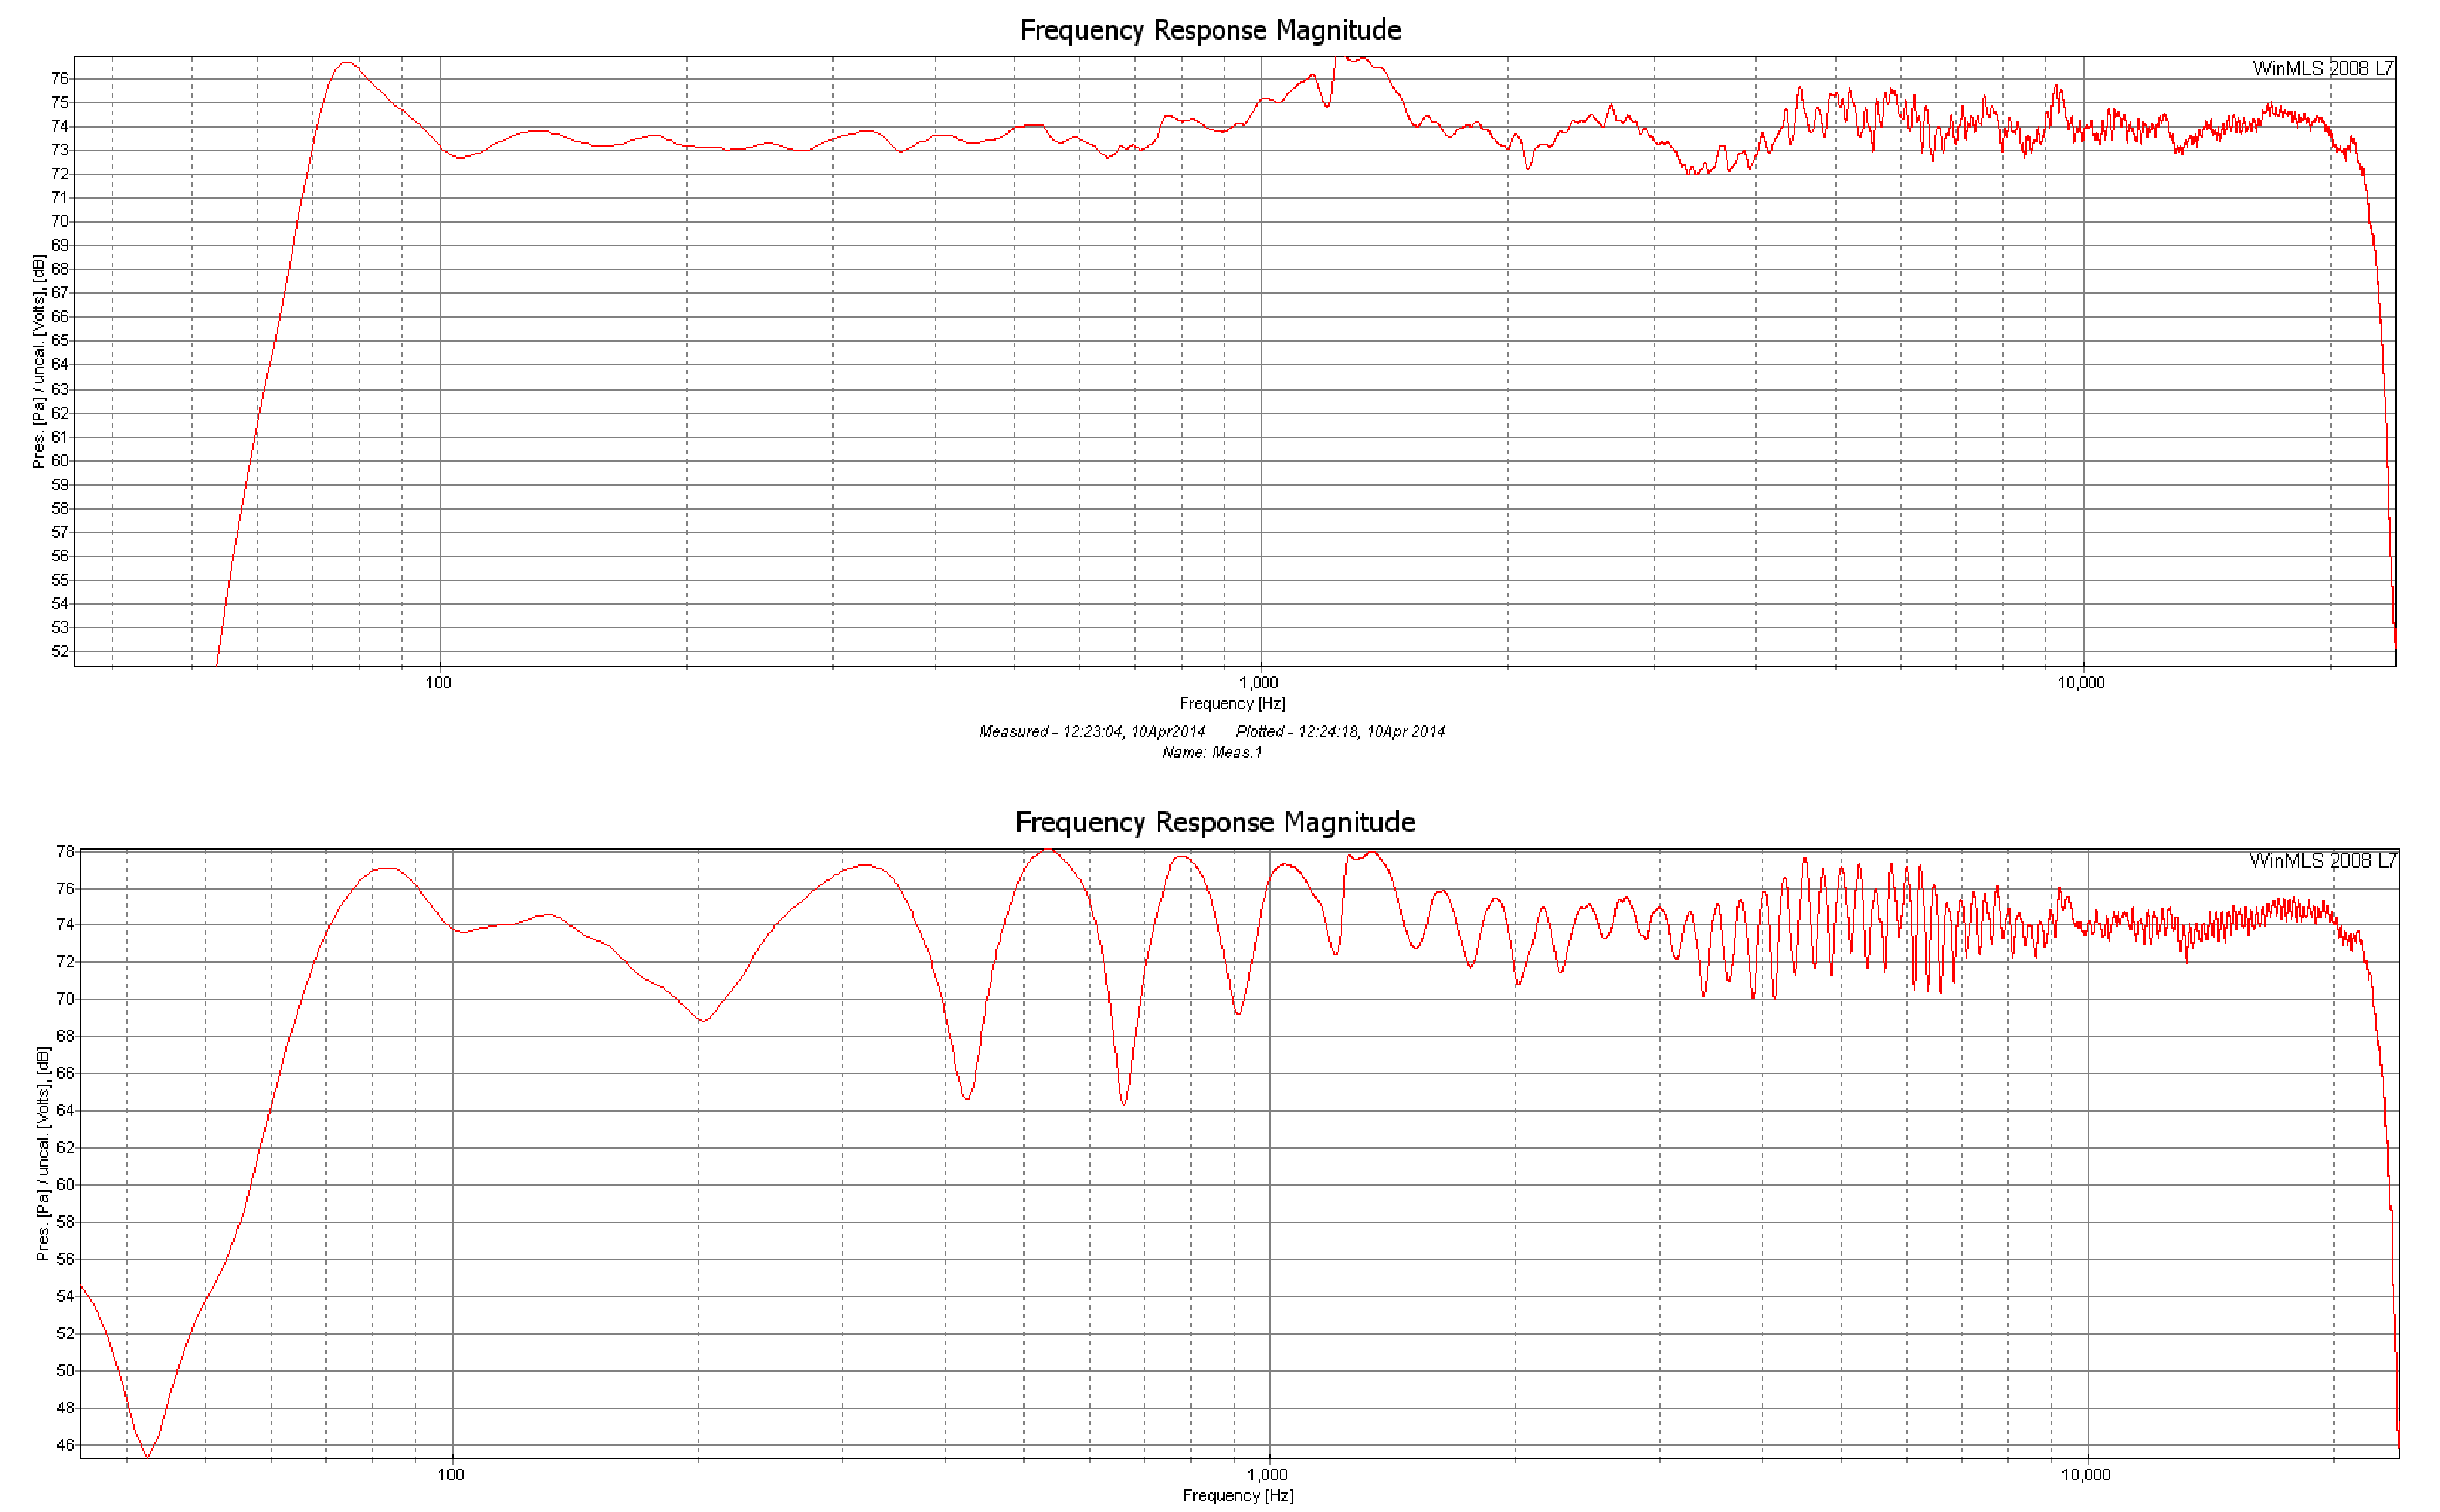
\includegraphics[width=15cm,keepaspectratio=true]{Figures/TaskC}
\caption{Frequency response (a) without and (b) with reflective surface}
\label{fig:TaskC}
\end{center}
\end{figure}

\newpage
\section{Conclusion}
In this laboratory measurements of loudspeaker parameters were done. Therefore a loudspeaker was placed on a turntable and put in front of a measurement microphone. This was done in an anechoic chamber. In a first measurement it can be obtained, that especially at low frequencies resulting frequency responses get wrong when the FFT time window is chosen too short. But in an other way the frequency response gets more smooth and less calculations have to be done. In a second step the directivity of the loudspeaker was measured. In this measurement it could be obtained that the directivity occurs mainly in higher frequencies, while at low frequencies the loudspeaker emits sound almost omnidirectional. The higher the frequency is the more directional the sound source becomes. In a last measurement the influence of reflections to the measurement was measured. Here it could be seen that reflections have huge interactions with the resulting frequency responses, large constructive and destructive interferences could be obrtained.

\newpage
\section*{References}
\footnotesize{
\begin{itemize}
\item Svensson, Peter, \textit{lecture notes}
\end{itemize}
}

\newpage
\appendix
\section{Example calculations}
\subsection{Efficiency}
\subsection{Sensitivity}
\subsection{Maximum output level}
\subsection{Measurement distance}
\subsection{Truncated impulse responses}
\subsection{Edge reflection/diffraction}


\section{Further plots}
\subsection{Frequency responses}
\end{document}
